% Chapter Template

\chapter{Parameter Estimation for ACWE Chan-Vese Segmentation} % Main chapter title

\label{chap:Chapter6} % Change X to a consecutive number; for referencing this chapter elsewhere, use \ref{ChapterX}

\textcolor{red}{[Introduction] What is special about the Chan-Vese formulation to the Mumford-Shah evolution energy function. Advantages, disadvantages (parameter estimation). Course of the chapter.}


\section{Graph Cut Model for Chan-Vese Segmentation}
\label{sec:chanveseGC}

\textcolor{red}{Chan-Vese formulation of the Mumford-Shah formulation. Length approximation using discrete representations (cut-metrics). Discrete representation of Chan-Vese formulation. Graph representation and sub-modularity constraint. Insensitivity to initialisation. What do the parameters mean and how do they influence the final result.}
In this section we briefly reintroduce the graph cut formulation for the Chan-Vese formulation of the Mumford-Shah evolution energy function for image segmentation. The Mumford-Shah model uses gradient descent techniques to obtain a minimum but as previously discussed, \Cref{sec:MAPMRFEstimation}, they usually terminate at local minima. By reformulating the energy function in a discrete form that allows for appropriate graph representability, we can use graph cuts, which are able to terminate at a global minimum, to iteratively converge to the optimal solution. For an in-depth exposition into this technique, look to \citep{Mumford1989,Chan2001,ElZehiry2007}.

The level set representation of the Mumford-Shah energy function is 
\begin{equation}
	\begin{split}
		F(c_1, c_2, \phi) & = \mu \int_\Omega \delta(\phi(x,y))|\nabla\phi(x,y)|dxdy \\
		& + \nu \int_\Omega H(\phi(x,y))dxdy \\
		& + \lambda_1 \int_\Omega |u(x,y)-c_1|^2H(\phi(x,y))dxdy \\
		& + \lambda_2 \int_\Omega |u(x,y)-c_2|^2(1-H(\phi(x,y)))dxdy,
	\end{split}
	\label{eq:mumfordshahfunction}
\end{equation}
where $u(x,y)$ is the image, $H(\cdot)$ is the Heaviside step function, $\delta(\cdot)$ is the Dirac delta function, $\phi:\Omega \rightarrow \Re$ is the level set function, such that:
\begin{equation}
	\begin{split}
		\omega & = \{(x,y) \in \Omega|\Phi(x_p)>0\} \text{ Inside the boundary} \\
		\bar{\omega} & = \{(x,y) \in \Omega|\Phi(x_p)<0\} \text{ Outside the boundary} \\
		C = \partial\omega & = \{(x,y) \in \Omega|\Phi(x_p)=0\} \text{ Along the boundary},
	\end{split}
	\label{eq:levelsetrepresentation}
\end{equation}
$c_1$ and $c_2$ are the arithmetic means given by:
\begin{equation}
	c_1(\phi) = \frac{\int_\Omega u(x,y)H(\phi(x,y))dxdy}{\int_\Omega H(\phi(x,y))dxdy},
	\label{eq:c1}
\end{equation}
\begin{equation}
c_2(\phi) = \frac{\int_\Omega u(x,y)(1-H(\phi(x,y)))dxdy}{\int_\Omega (1-H(\phi(x,y)))dxdy}.
\label{eq:c2}
\end{equation}
The piecewise smooth approximation of the image is then 
\begin{equation}
	u(x,y) = c_1 H(\phi(x,y)) + c_2(1-H(\phi(x,y))).
	\label{eq:piecewiseapproximation}
\end{equation}

\begin{definition}[Discrete Approximation of Contour Length]
	For the energy function to be represented as a graph, one of the requirements is that it must be in a discrete representation. This means that the length of the contour, the first term in \Cref{eq:mumfordshahfunction}, must be approximated discretely and be graph representable. This work has already been done by Kolmogorov and Boykov in \citep{Kolmogorov2005_2,Boykov2003} where they used the Cauchy-Crofton thereom. The thereom states that the length of a curve can be approximated by draw a large number of straight lines from $0$ to $2\pi$ and counting the number of intersections between the lines and the contour. The mathematical representation is
	\begin{equation}
		\int_L n_L dL = \int_{0}^{\pi}\int_{-\infty}^{\infty} n_L d\rho d\theta = 2 \lVert C \rVert_E,
	\end{equation}
	where $n_L$ is the number of intersections between the contour $C$ and the line $L$, $ \lVert C \rVert_E$ is the Euclidean length of the contour, $0 < \rho < \infty$ and $0 < \theta < 2\pi$. From this the discrete approximation used by Boykov and Zabih is 
	\begin{equation}
		\lVert C \rVert_E = \frac{1}{2}\sum_k n_k \frac{\delta^2 \Delta\theta_k}{|e_k|} = \frac{1}{2}\sum_k n_k w_k
		\label{eq:discretelength}
	\end{equation}
\end{definition}
An example of approximating the contour by two grids is illustrated in \Cref{fig:chanveselength} using four families of parallel lines which are $45^\text{o}$ apart.

\begin{figure}[!t]
	\centering
	\subfigure[]
	{
		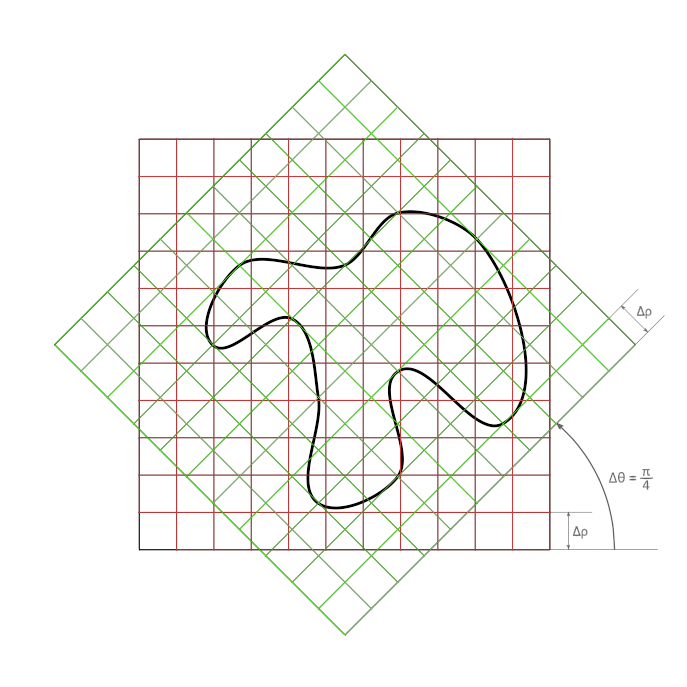
\includegraphics[width=0.45\columnwidth]{chan_vese_length.png}
		\label{fig:chanveselength}
	}
	\subfigure[]
	{
		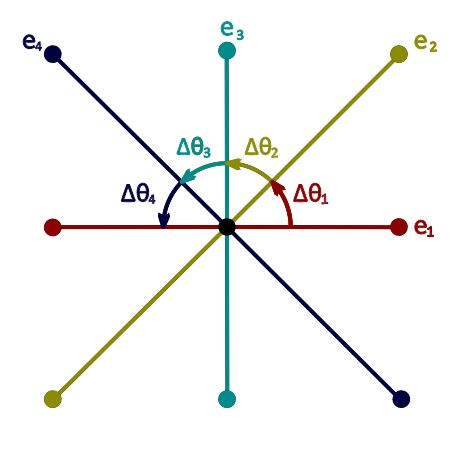
\includegraphics[width=0.45\columnwidth]{chan_vese_cauchycrofton.png}
		\label{fig:chanvesediscretelength}
	}
	\caption{\textbf{(a)} Cauchy-Crofton length approximation. \textbf{(b)} 8-connected neighbourhood system.}
	\label{fig:chanveseN8}
\end{figure}

\begin{definition}[Discrete Representation of Mumford-Shah Function]
	With the exception of the second term in \Cref{eq:mumfordshahfunction}, the remaining terms are represented easily discretely. For each pixel $p \in \Omega$, let $x_p$ be a binary variable such that
	\begin{equation}
		x_p = 
		\begin{cases} 
			0 & \phi(p)\leq 0 \\
			1 & \phi(p)> 0
		\end{cases}
	\end{equation}
	The means can now be calculated using 
	\begin{equation}
		c_1 = \frac{\sum_p u(x,y)x_p}{\sum_p x_p},
	\end{equation}
	\begin{equation}
		c_2 = \frac{\sum_p u(x,y)(1-x_p)}{\sum_p (1-x_p)}.
	\end{equation}
	For simplification, $\nu=0$. To determine contour length using an 8-neighbourhood system, as illustrated in \Cref{fig:chanvesediscretelength}, we set $\Delta\rho=1$. The weight $w_k$ is assigned to it's corresponding edge $e_k$. The Euclidean length of the  edges is $|e_1|=|e_3| = 1$ and $|e_2|=|e_4|=\sqrt{2}$, therefore the corresponding weights, which are determined using \Cref{eq:discretelength}, is $w_1 = w_3 = \frac{\pi}{8}$ and $w_2 = w_4 = \frac{\pi}{8\sqrt{2}}$. To calculate $n_k$ we need to count the intersections between the lines and the contour. An intersection between two pixels $p$ and $q$ exists \textit{if and only if} $x_p$ and $x_q$ have different labels.
	\begin{equation}
		n_{k} = x_p(1-x_q) + x_q(1-x_p) \text{; } \, k={(pq) \in \mathcal{N}_p}. 
	\end{equation}
	The contour length can now fully be expressed discretely as 
	\begin{equation}
		\lVert C \rVert_E = \sum_{p,q \in e_k} w_k( x_p(1-x_q) + x_q(1-x_p)).
	\end{equation}
	
	The discrete representation of \Cref{eq:mumfordshahfunction} is
	\begin{equation}
		\begin{split}
			F(x_1, \ldots, x_n) & = \mu \sum_{p,q \in e_k} w_k( x_p(1-x_q) + x_q(1-x_p)) \\
			& + \lambda_1 \sum_p |u(x,y)-c_1|^2x_p \\
			& + \lambda_2 \sum_p |u(x,y)-c_2|^2(1-x_p)
		\end{split}
		\label{eq:discretemumfordshah}
	\end{equation}
\end{definition}

\begin{definition}[Graph Representation] The discrete energy function \Cref{eq:discretemumfordshah} has been shown that it obey the submodularity constraint for graph representability. Therefore the data energy and regularistion energy is
	\begin{equation}
		E^p(x_p) = \lambda_1 |u(x,y)-c_1|^2 x_p + \lambda_2 |u(x,y)-c_2|^2 (1-x_p)
	\end{equation}
	\begin{equation}
	E^{pq}(x_p,x_q) = (x_p + x_q - 2x_px_q)w_{pq}
	\end{equation}
\end{definition}
The graph for the energy function is constructed as in \citep{Kolmogorov2004}.

\section{Modified Weighting and Parameter Estimation}
\label{sec:cvgc_weightingandparameterestimation}

\textcolor{red}{What is wrong with the previously described graph weighting. What would we expect from a better weighting system.}

\subsection{Weighting}
\label{sec:cvgc_weighting}

\textcolor{red}{Describe the modified weighting and parameter relations.}

\subsection{Analysis of Weighting System and Parameter Relationships}
\label{sec:cvgc_analysis}

\textcolor{red}{Describe the relationship between various parameters including their limits and ranges.}

\subsection{Tuning Parameters for Fluorescence Microscopy}
\label{sec:cvgc_parameterestimation}

\textcolor{red}{What sort of image properties are we tuning for? E.g. dark bg, low contrast, etc. Parameters limits and ranges.}

\section{Experimental Results}
\label{sec:cvgc_experimentalresults}

\textcolor{red}{Present and analyse the experimental results.}
